\section{Experiments and results}\label{sec:chp6:exp-res}



In this section, we present a variety to validate out \ac{mpmri} \ac{cad} for the detection of \ac{cap}.
Table~\ref{tab:exp-summary} represents the summary of the experiments. 
These experiments and the results obtained are discussed in details in the reminder of this section. 
Pre-processing, segmentation and registration of each modalities are common steps across all the designed experiments.

\subsection{Experiment-1: Assessment of inidivual modalities}\label{subec:chp6:exp-res:Ex1} 
The main goal of this experiment is to eavluate the potential of each inividual modality and their corresponding features. 
Different features as presented in Sect.~\ref{subsec:chp6:method:fea-det} are extracted for different modalities. 
For all the modalities, the extracted features without any extraction or selection process are used to train a \ac{rf} classifier, using a \ac{lopo}. 
These experiments are performed using {\color{red} which dataset}.
The results are presented in terms of \ac{roc} analysis and averaged \ac{auc} over \ac{lopo}.
Figure~\ref{fig:res-Ex1} illustrate the obtained results.

\begin{figure}
  \hspace*{\fill}
  \subfigure[Performance of the quantitative methods on \acs*{dce}-\acs*{mri}.]{\label{fig:}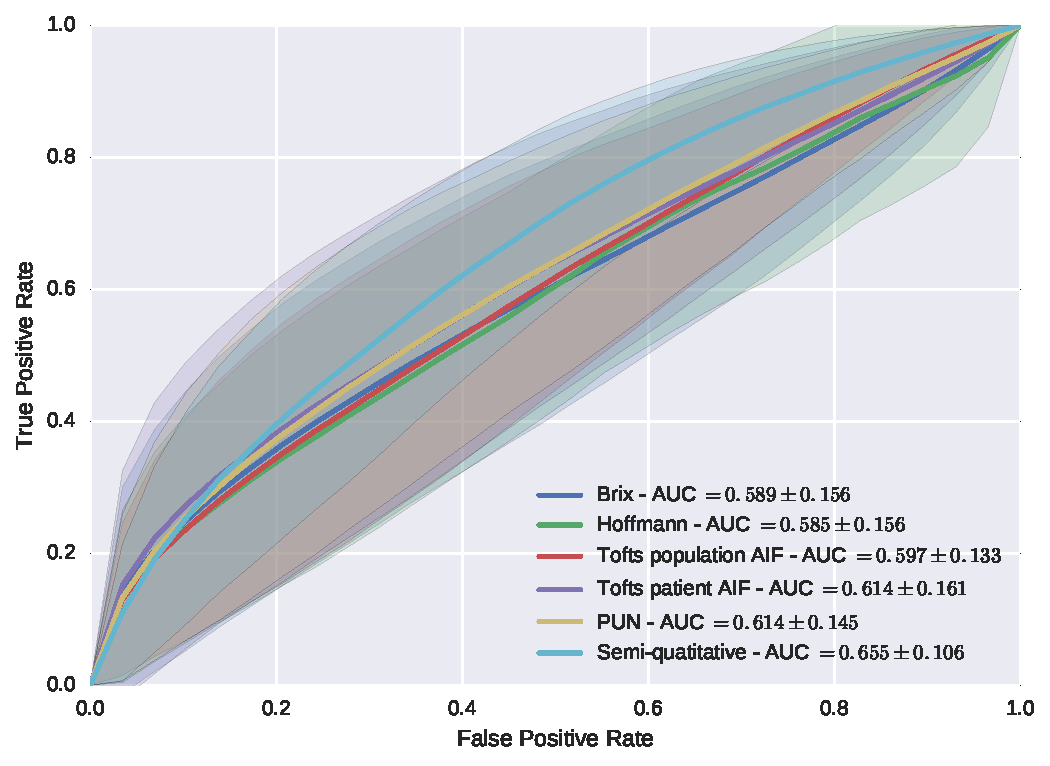
\includegraphics[width=.49\textwidth]{5_normalization/figures/DCE-normalization/normalized_methods_0.pdf}}
  \hfill
  \subfigure[Performance of enhanced \acs*{dce}-\acs*{mri} signal.]{\label{fig:}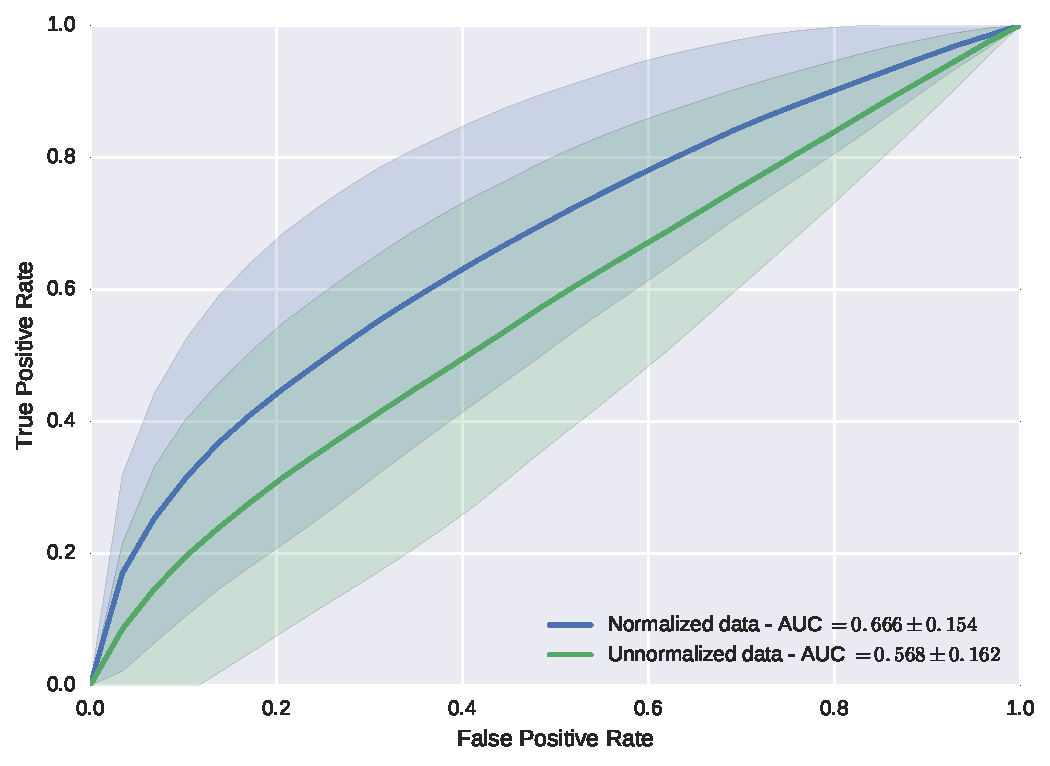
\includegraphics[width=.49\textwidth]{5_normalization/figures/DCE-normalization/full_signal_0.pdf}}
  \hspace*{\fill} \\
  \hspace*{\fill}
  \subfigure[Performance of image-based features for \acs*{t2w}-\acs*{mri} and \acs*{adc} map.]{\label{fig:}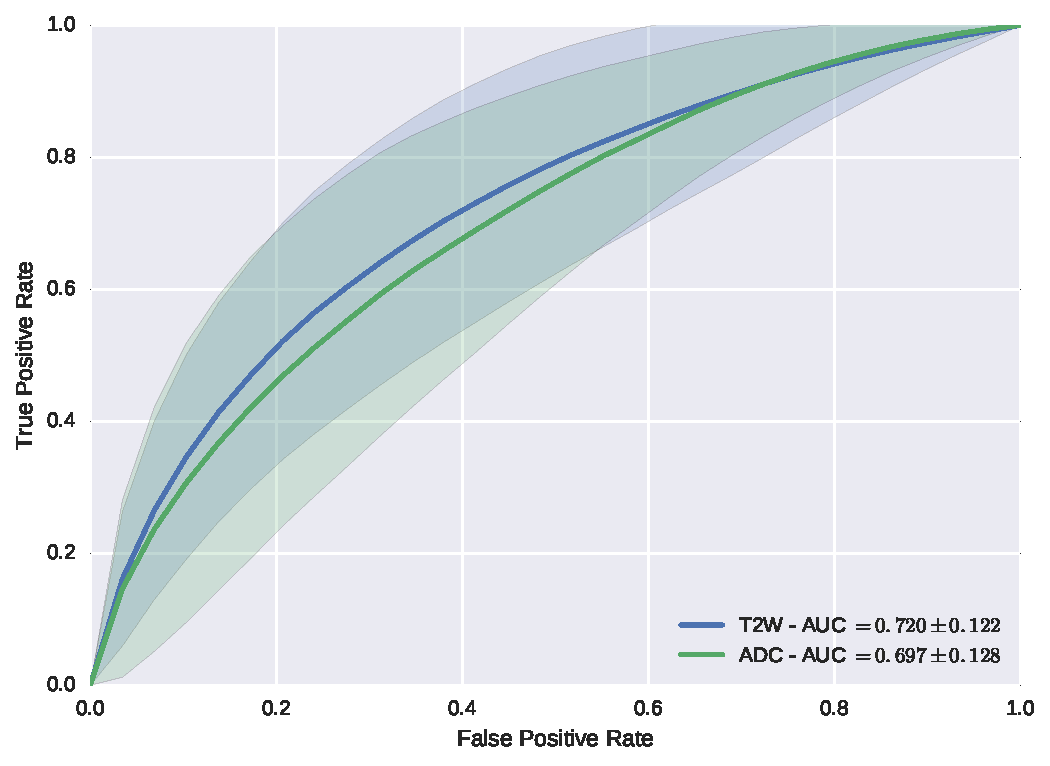
\includegraphics[width=.49\textwidth]{6_pipeline/figures/exp-1/t2w_adc.pdf}}
  \hfill
  \subfigure[Performance of different approach for the \acs*{mrsi} modality.]{\label{fig:}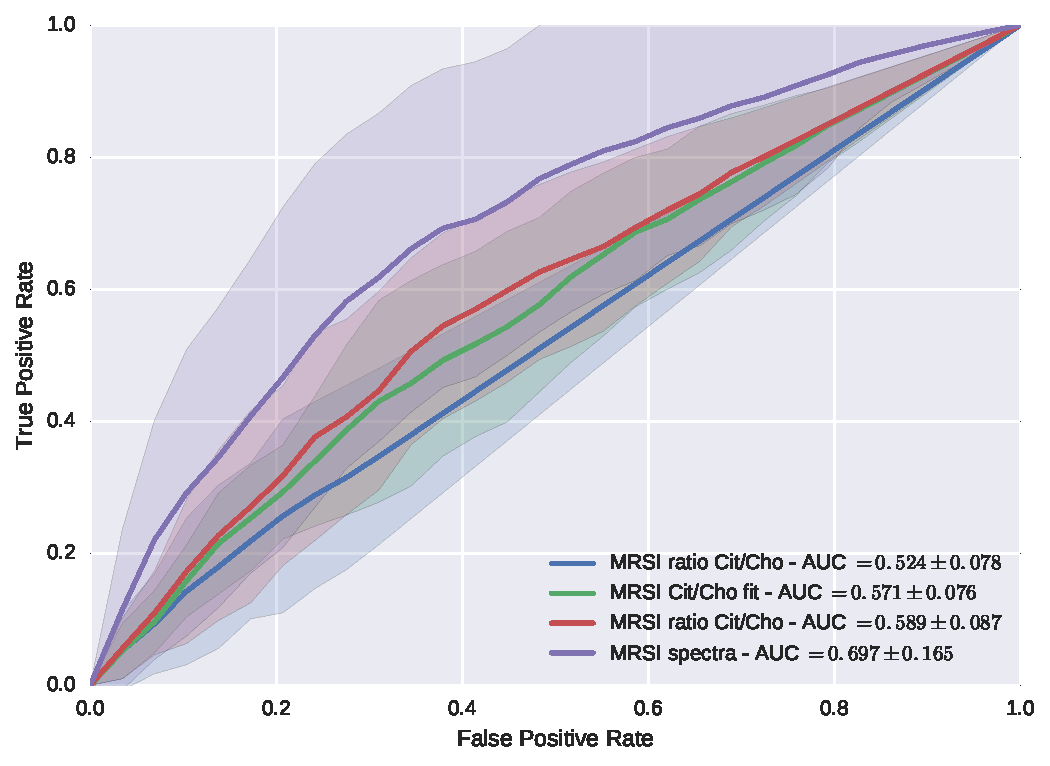
\includegraphics[width=.49\textwidth]{6_pipeline/figures/exp-1/mrsi_all.pdf}}
  \hspace*{\fill}
  \caption[Analysis of the classification performance for each individual \acs*{mri} modality.]{Analysis of the classification performance for each individual \acs*{mri} modality.}
  \label{fig:res-Ex1}
\end{figure}


\subsection{Experiment-2: Coarse combination} \label{subsec:chp6:exp-res:Ex2}
The objective of this experiment is to evaluate the combination of all the modalities.
To this extent, three different approaches are considered: (i) feature aggregation, (ii) statcking using \ac{adb}, (iii) stacking using \ac{gb}. 
In the first approach, feature aggregation, the features extracted from each modalities (\ac{t2w}, \ac{adc}, normalized-whole-\ac{dce} and normalized-whole-\ac{mrsi}, as concluded in experiment-1) are concatenated together and used with a \ac{rf} classifier and \ac{lopo}. 
In the second and third approach since stacking is used the training set is divided into training and validation set.
Therefore, first a \ac{rf} classifier is trained for each modality using the their corresponding training set and then using a validation set their prediction is fed as a training to a meta learner.
\Ac{adb} and \ac{gb} are used as a meta learner for the second and third approach, respectively. 
Figure~\ref{fig:flow-Ex2} shows the framework of the first and second/third approach. 

The obtained results of this experiment are shown in Fig.~\ref{fig:res-Exp2}.
\begin{figure}
  \centering
  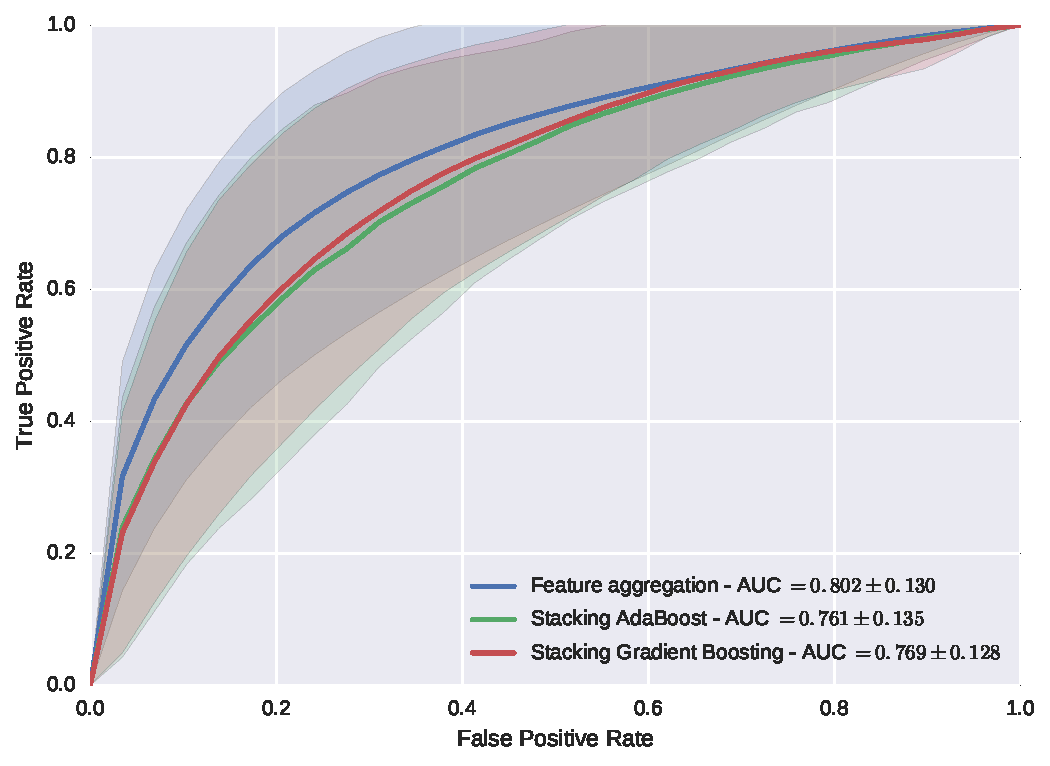
\includegraphics[width=0.8\linewidth]{6_pipeline/figures/exp-2/comb_all.pdf}
  \caption[Comparison of different combination approaches.]{Comparison of different combination approaches: (i) aggregation of the different features in conjunction with a \acs*{rf} classifier, (ii) a stacking approach using 4 \acs*{rf}s and \acs*{adb} as meta-classifier, and (iii) a stacking approach using 4 \acs*{rf}s and \acs*{gb} as meta-classifier.}
  \label{fig:res-Exp2}
\end{figure}

\subsection{Experiment-3: Fine tuning}\label{subsec:chp6:exp-res:Ex3}
In the previous experiments (1 \& 2) the original features were used, without any adjustment or tunning. 
In this section, as we call it fine tuning, first we evaluate the performance and benefits of having a balance set, then we eavaluate different feature selection and extraction techniques.
The main aim of this experiment is to find the best balancing technique and feature selection approach suited for each modality. 
Therefore, simiar to experiment-1, only the performance of individual modalities are comapered. 

The \ac{us1} and \ac{os} techniques used to balance our training set were explained in Sect.~\ref{subsec:chp6:method:fea-bal}.
Figure~\ref{fig:res-Ex3-bal} shows the comparison of these techniques on each modality. 
\begin{figure}
  \hspace*{\fill}
  \subfigure[\ac{t2w}-\ac{mri}]{\label{fig:ex3:T2W}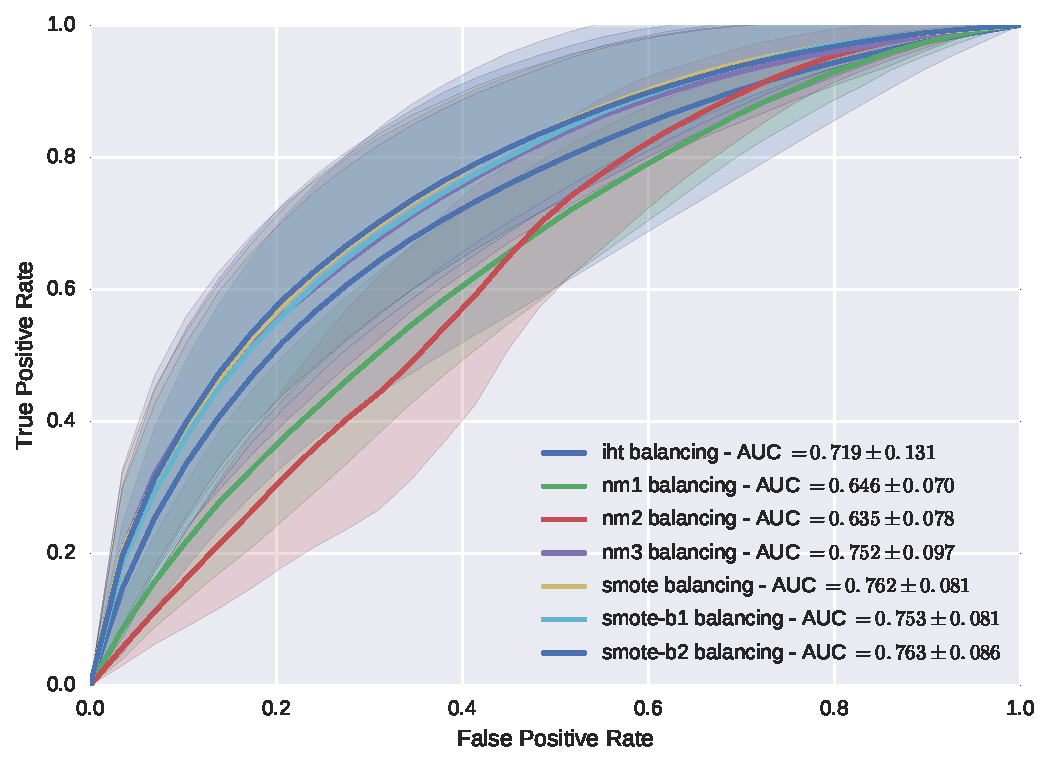
\includegraphics[width=.49\textwidth]{6_pipeline/figures/exp-3/t2w.pdf}}
  \hfill
  \subfigure[\ac{adc}-\ac{mri}]{\label{fig:ex3:ADC}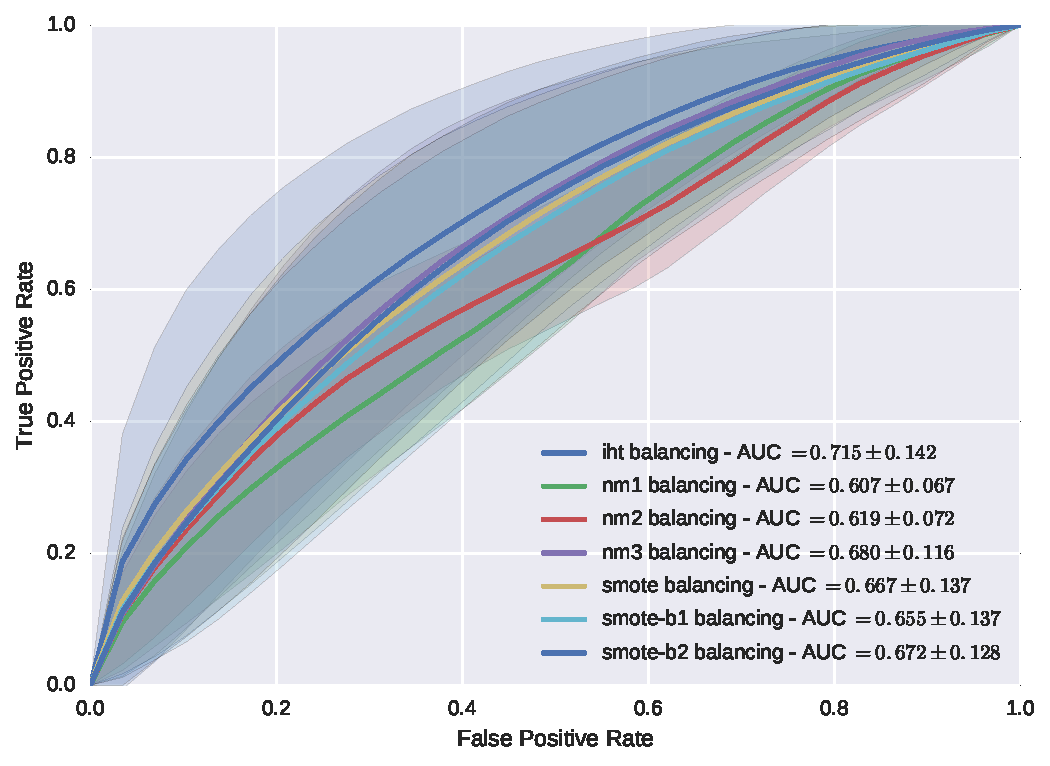
\includegraphics[width=.49\textwidth]{6_pipeline/figures/exp-3/adc.pdf}}
  \hspace*{\fill} \\
  \hspace*{\fill}
  \subfigure[\ac{dce}-\ac{mri}]{\label{fig:ex3-DCE}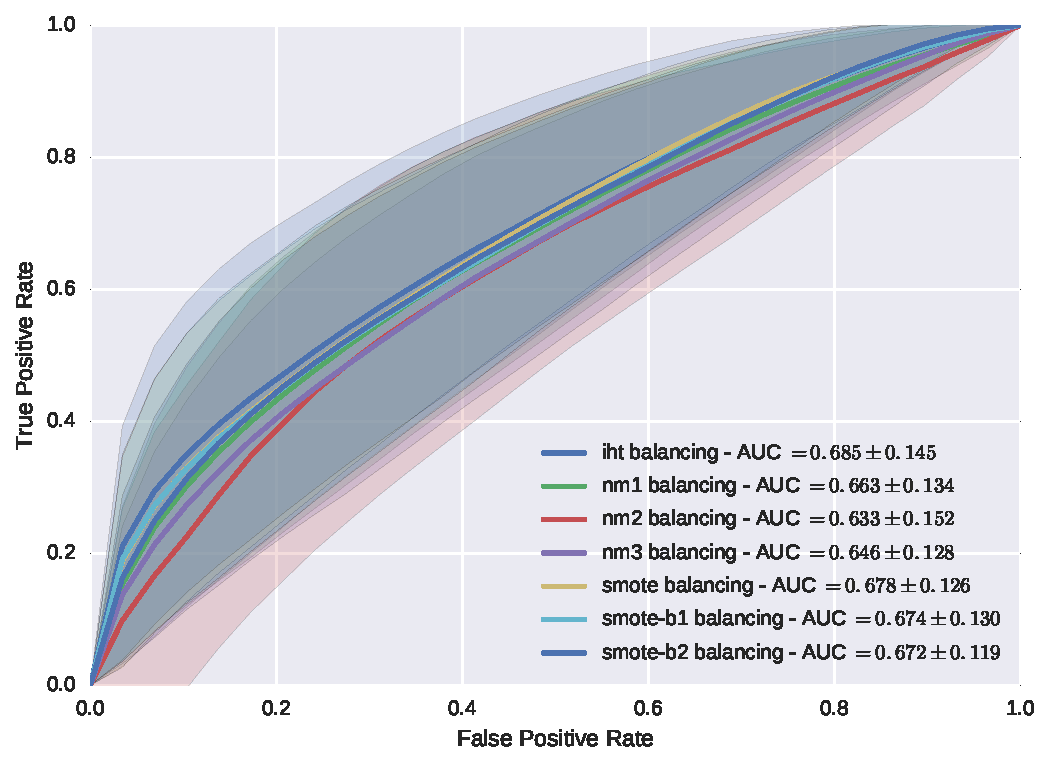
\includegraphics[width=.49\textwidth]{6_pipeline/figures/exp-3/dce.pdf}}
  \hfill
  \subfigure[\ac{mrsi}-\ac{mri}]{\label{fig:ex3-MRSI}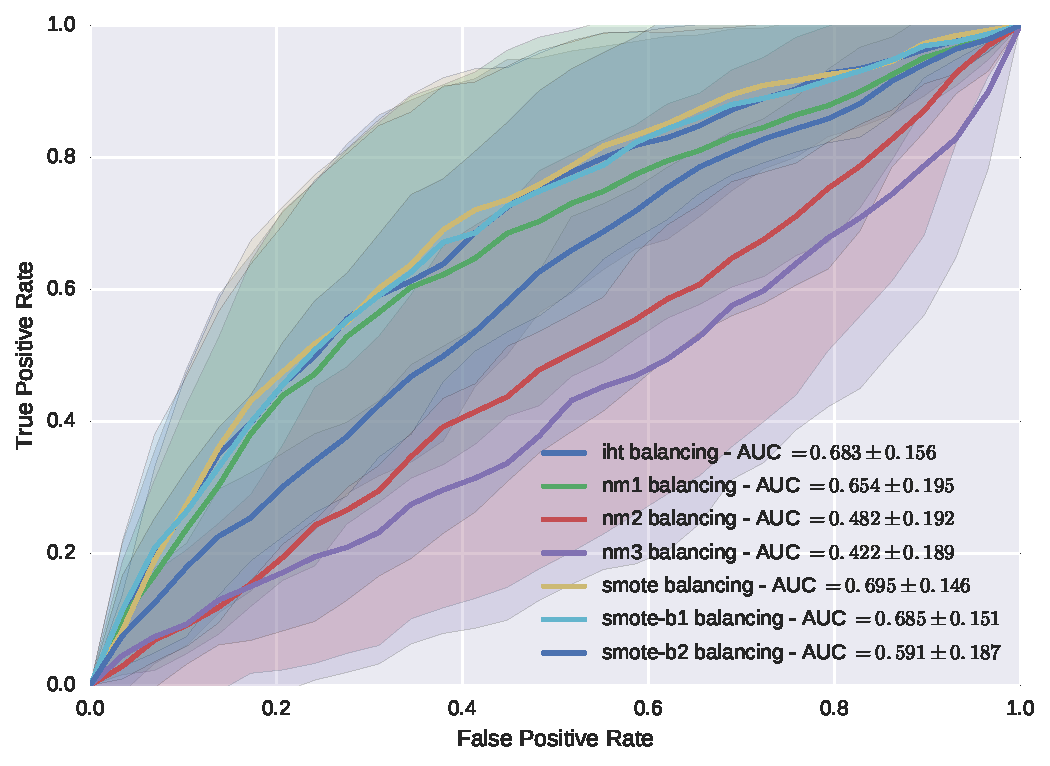
\includegraphics[width=.49\textwidth]{6_pipeline/figures/exp-3/mrsi.pdf}}
  \hspace*{\fill}
  \caption[Analysis of the benefit of balancing the training dataset before learning process.]{Analysis of the benefit of balancing the training dataset before learning process.}
  \label{fig:res-Ex3-bal}
\end{figure}


\begin{landscape}

\begin{table}
  \caption{Results in terms of \acs*{auc} of the feature selection based on \acs*{anova} F-value for \acs*{t2w}-\acs*{mri}.}
  \centering
  \scriptsize
  \begin{tabularx}{\linewidth}{@{}l >{\centering\arraybackslash}X >{\centering\arraybackslash}X >{\centering\arraybackslash}X >{\centering\arraybackslash}X >{\centering\arraybackslash}X >{\centering\arraybackslash}X >{\centering\arraybackslash}X @{}}
    \toprule
    \textbf{Methods} & \multicolumn{7}{c}{\textbf{Percentiles}} \\
    \cmidrule{2-8}
    & 15 & 17.5 & 20 & 22.5 & 25 & 27.5 & 30 \\
    \midrule
    \acs*{anova} F-score & $0.755 \pm 0.049$ & $0.770 \pm 0.058$ & $0.777 \pm 0.064$ & $0.782 \pm 0.066$ & $\mathbf{0.784 \pm 0.067}$ & $0.783 \pm 0.072$ & $0.782 \pm 0.070$ \\
    \bottomrule
  \end{tabularx}
  \label{tab:ginit2w}
\end{table}

\begin{table}
  \caption{Results in terms of \acs*{auc} of the feature selection based on Gini importance for \acs*{t2w}-\acs*{mri}.}
  \centering
  \scriptsize
  \begin{tabularx}{\linewidth}{@{}l >{\centering\arraybackslash}X >{\centering\arraybackslash}X >{\centering\arraybackslash}X >{\centering\arraybackslash}X >{\centering\arraybackslash}X >{\centering\arraybackslash}X >{\centering\arraybackslash}X @{}}
    \toprule
    \textbf{Methods} & \multicolumn{7}{c}{\textbf{Percentiles}} \\
    \cmidrule{2-8}
    & 1 & 2 & 5 & 10 & 15 & 20 & 30 \\
    \midrule
    Gini importance & $0.726 \pm 0.064$ & $0.731 \pm 0.055$ & $0.751 \pm 0.065$ & $0.758 \pm 0.076$ & $0.752 \pm 0.087$ & $0.761 \pm 0.077$ & $\mathbf{0.764 \pm 0.079}$ \\
    \bottomrule
  \end{tabularx}
  \label{tab:anovat2w}
\end{table}

\begin{table}
  \caption{Results in terms of \acs*{auc} of the feature selection based on \acs*{anova} F-value for \acs*{adc}.}
  \centering
  \scriptsize
  \begin{tabularx}{\linewidth}{@{}l >{\centering\arraybackslash}X >{\centering\arraybackslash}X >{\centering\arraybackslash}X >{\centering\arraybackslash}X >{\centering\arraybackslash}X >{\centering\arraybackslash}X >{\centering\arraybackslash}X @{}}
    \toprule
    \textbf{Methods} & \multicolumn{7}{c}{\textbf{Percentiles}} \\
    \cmidrule{2-8}
    & 10 & 12.5 & 15 & 17.5 & 20 & 22.5 & 25 \\
    \midrule
    \acs*{anova} F-score & $0.684 \pm 0.123$ & $0.713 \pm 0.125$ & $0.712 \pm 0.134$ & $0.710 \pm 0.144$ & $\mathbf{0.714 \pm 0.142}$ & $0.708 \pm 0.150$ & $0.708 \pm 0.150$ \\
    \bottomrule
  \end{tabularx}
  \label{tab:giniadc}
\end{table}

\begin{table}
  \caption{Results in terms of \acs*{auc} of the feature selection based on Gini importance for \acs*{adc} map.}
  \centering
  \scriptsize
  \begin{tabularx}{\linewidth}{@{}l >{\centering\arraybackslash}X >{\centering\arraybackslash}X >{\centering\arraybackslash}X >{\centering\arraybackslash}X >{\centering\arraybackslash}X >{\centering\arraybackslash}X >{\centering\arraybackslash}X @{}}
    \toprule
    \textbf{Methods} & \multicolumn{7}{c}{\textbf{Percentiles}} \\
    \cmidrule{2-8}
    & 1 & 2 & 5 & 10 & 15 & 20 & 30 \\
    \midrule
    Gini importance & $0.672 \pm 0.132$ & $0.690 \pm 0.138$ & $\mathbf{0.743 \pm 0.139}$ & $0.730 \pm 0.136$ & $0.730 \pm 0.142$ & $0.724 \pm 0.141$ & $0.722 \pm 0.142$ \\
    \bottomrule
  \end{tabularx}
  \label{tab:anovaadc}
\end{table}

\begin{table}
  \caption{Results in terms of \acs*{auc} of the feature extraction methods for \acs*{dce}-\ac{mri}.}
  \centering
  \scriptsize
  \begin{tabularx}{\linewidth}{@{}l >{\centering\arraybackslash}X >{\centering\arraybackslash}X >{\centering\arraybackslash}X >{\centering\arraybackslash}X >{\centering\arraybackslash}X >{\centering\arraybackslash}X >{\centering\arraybackslash}X @{}}
    \toprule
    \textbf{Methods} & \multicolumn{7}{c}{\textbf{Number of components or sparsity level}} \\
    \cmidrule{2-8}
    & 2 & 4 & 8 & 16 & 24 & 32 & 36 \\
    \midrule
    \acs*{pca} & $0.656 \pm 0.133$ & $0.634 \pm 0.121$ & $0.668 \pm 0.149$ & $0.680 \pm 0.145$ & $0.682 \pm 0.146$ & $0.679 \pm 0.151$ & $0.683 \pm 0.149$ \\
    Sparse-\acs*{pca} & $0.578 \pm 0.117$ & $0.546 \pm 0.121$ & $0.554 \pm 0.097$ & --- & --- & --- & --- \\
    \acs*{ica} & $0.657 \pm 0.132$ & $0.629 \pm 0.117$ & $0.671 \pm 0.157$ & $0.686 \pm 0.158$ & $\mathbf{0.691 \pm 0.158}$ & $0.681 \pm 0.161$ & $0.679 \pm 0.166$ \\
    \bottomrule
  \end{tabularx}
  \label{tab:dcefeatext}
\end{table}


\begin{table}
  \caption{Results in terms of \acs*{auc} of the feature extraction methods for \acs*{mrsi}.}
  \centering
  \scriptsize
  \begin{tabularx}{\linewidth}{@{}l >{\centering\arraybackslash}X >{\centering\arraybackslash}X >{\centering\arraybackslash}X >{\centering\arraybackslash}X >{\centering\arraybackslash}X >{\centering\arraybackslash}X >{\centering\arraybackslash}X @{}}
    \toprule
    \textbf{Methods} & \multicolumn{7}{c}{\textbf{Number of components or sparsity level}} \\
    \cmidrule{2-8}
    & 2 & 4 & 8 & 16 & 24 & 32 & 36 \\
    \midrule
    \acs*{pca} & $0.566 \pm 0.120$ & $0.575 \pm 0.141$ & $0.648 \pm 0.162$ & $0.662 \pm 0.177$ & $0.659 \pm 0.184$ & $0.671 \pm 0.179$ & $0.672 \pm 0.182$ \\
    Sparse-\acs*{pca} & $0.502 \pm 0.050$ & $0.571 \pm 0.158$ & $0.585 \pm 0.111$ & --- & --- & --- & --- \\
    \acs*{ica} & $0.567 \pm 0.119$ & $0.578 \pm 0.140$ & $0.654 \pm 0.145$ & $0.656 \pm 0.167$ & $0.650 \pm 0.187$ & $0.663 \pm 0.174$ & $\mathbf{0.677 \pm 0.171}$ \\
    \bottomrule
  \end{tabularx}
  \label{tab:mrsifeatext}
\end{table}


\end{landscape}

\subsection{Experiment-4: Fine combination}\label{subsec:chp6:exp-res:Ex4}
This experiments evaluates the combination of all the modalities after applying fine tunning and adjusting the feature space. 
Two different approaches are compared: (i) Feature aggregation and (ii) stacking using \ac{gb}. 
The second approach of experiment-2 was ignored, since as previously concluded, \ac{gb} had a slightly better performance than \ac{adb}.

\begin{figure}
  \centering
  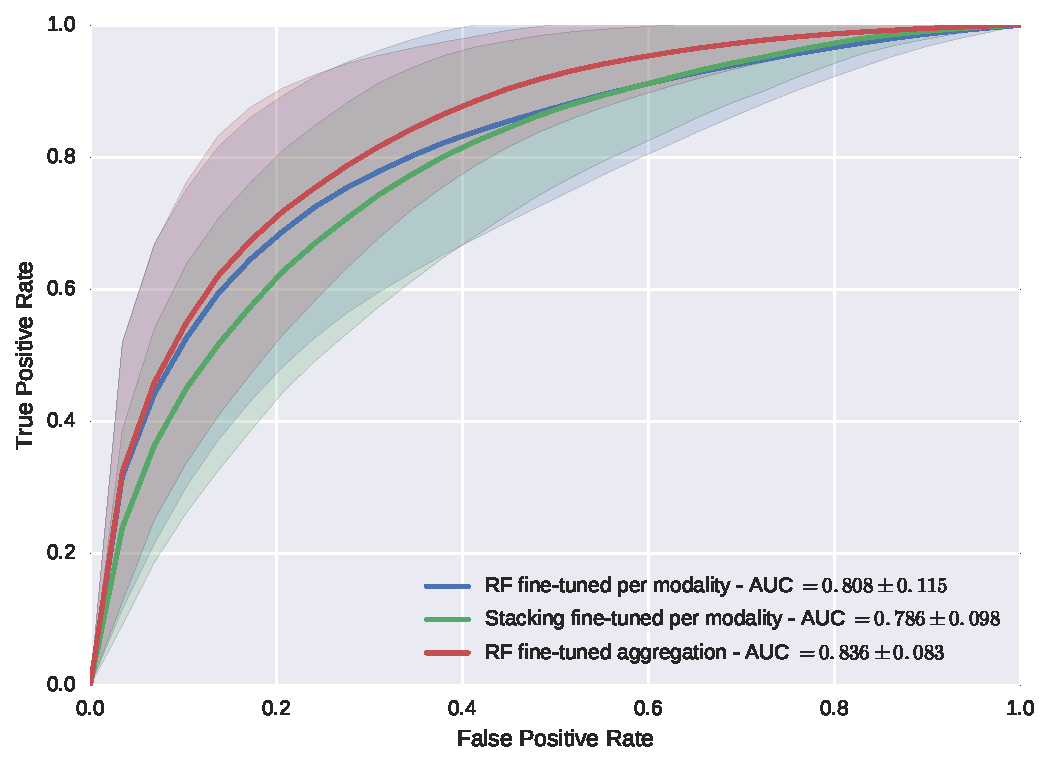
\includegraphics[width=0.7\linewidth]{6_pipeline/figures/exp-5/combine_all.pdf}
  \caption[Analysis of feature combination approaches after fine tuning.]{Analysis of feature combination approaches after fine tuning through balancing and feature selection/extraction.}
  \label{fig:res-Ex4}
\end{figure}


\begin{landscape}
\begin{table}
  \caption{Results in terms of \acs*{auc} of the feature selection based on \acs*{anova} F-value for the aggregation of feature from all \acs*{mpmri} features.}
  \centering
  \scriptsize
  \begin{tabularx}{\linewidth}{@{}l >{\centering\arraybackslash}X >{\centering\arraybackslash}X >{\centering\arraybackslash}X >{\centering\arraybackslash}X >{\centering\arraybackslash}X >{\centering\arraybackslash}X >{\centering\arraybackslash}X @{}}
    \toprule
    \textbf{Methods} & \multicolumn{7}{c}{\textbf{Percentiles}} \\
    \cmidrule{2-8}
    & 5 & 7.5 & 10 & 12.5 & 15 & 17.5 & 20 \\
    \midrule
    \acs*{anova} F-score & $0.771 \pm 0.133$ & $0.783 \pm 0.144$ & $0.789 \pm 0.133$ & $0.822 \pm 0.114$ & $\mathbf{0.822 \pm 0.112}$ & $0.817 \pm 0.113$ & $0.810 \pm 0.120B$ \\
    \bottomrule
  \end{tabularx}
  \label{tab:ginicomb}
\end{table}

\begin{table}
  \caption{Results in terms of \acs*{auc} of the feature selection based on Gini importance for the aggregation of feature from all \acs*{mpmri} features.}
  \centering
  \scriptsize
  \begin{tabularx}{\linewidth}{@{}l >{\centering\arraybackslash}X >{\centering\arraybackslash}X >{\centering\arraybackslash}X >{\centering\arraybackslash}X >{\centering\arraybackslash}X >{\centering\arraybackslash}X >{\centering\arraybackslash}X @{}}
    \toprule
    \textbf{Methods} & \multicolumn{7}{c}{\textbf{Percentiles}} \\
    \cmidrule{2-8}
    & 1 & 2 & 5 & 7.5 & 10 & 12.5 & 15 \\
    \midrule
    Gini importance & $0.773 \pm 0.142$ & $0.827 \pm 0.099$ & $0.822 \pm 0.105$ & $0.823 \pm 0.101$ & $\mathbf{0.831 \pm 0.100}$ & $0.816 \pm 0.113$ & $0.816 \pm 0.115$ \\
    \bottomrule
  \end{tabularx}
  \label{tab:anovacomb}
\end{table}

\end{landscape}

\begin{figure}
  \centering
  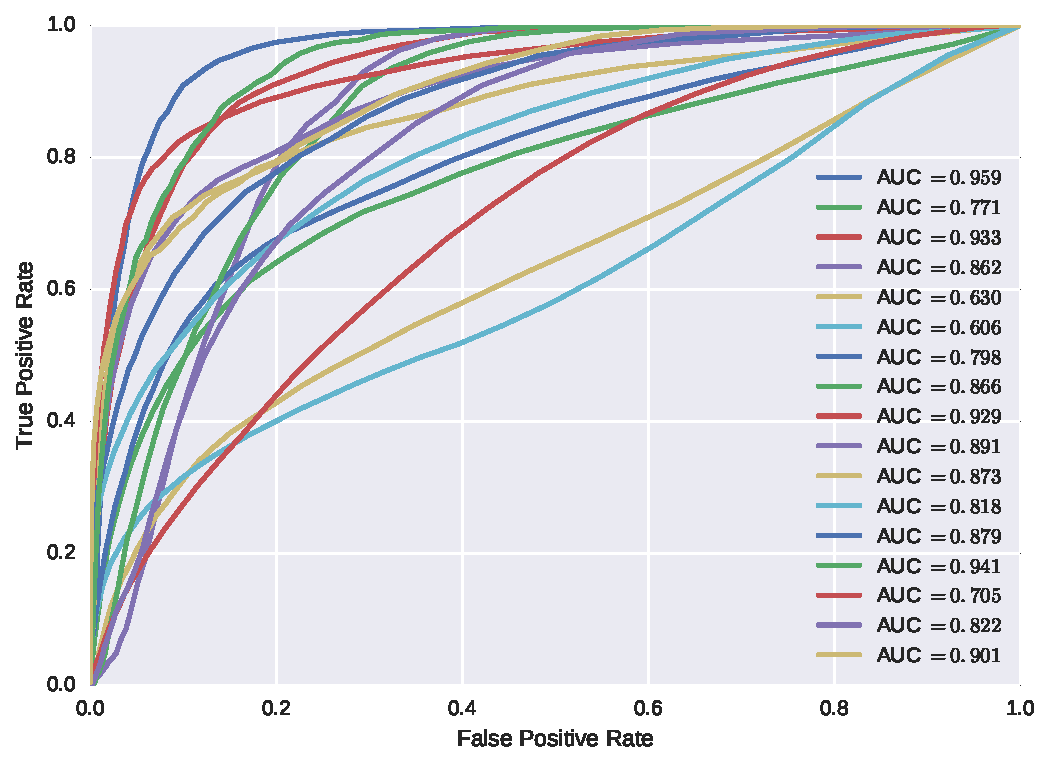
\includegraphics[width=0.7\linewidth]{6_pipeline/figures/exp-5/plot_all_patients.pdf}
  \caption{Individual patient \acs*{auc} for the best configuration of the \acs*{mpmri} \acs*{cad}.}
  \label{fig:indauc}
\end{figure}

\begin{figure}
  \centering
  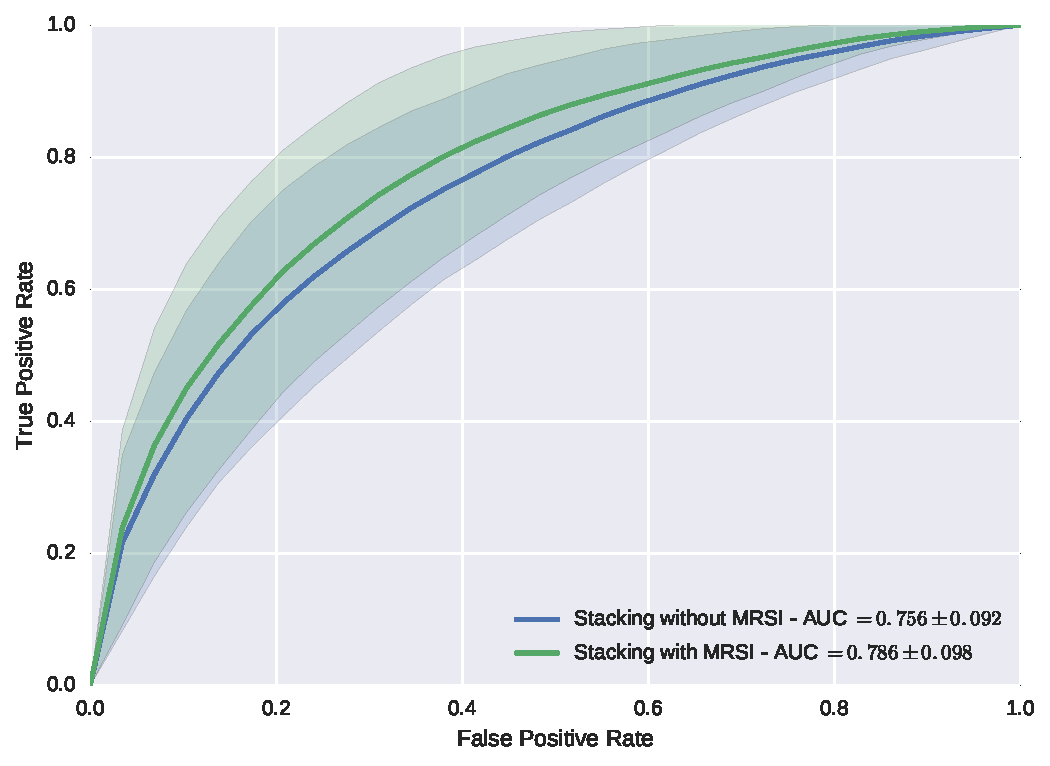
\includegraphics[width=0.7\linewidth]{6_pipeline/figures/exp-6/stacking_wt_mrsi.pdf}
  \caption{Illustration of the gain of including the \acs*{mrsi} modality in a \acs*{mpmri} \acs*{cad}.}
  \label{fig:resmrsigain}
\end{figure}
